\subsection{Das euklidische Pfadintegral} 
	\begin{align*}
		S= \int_{-\infty}^{\infty} \diff t ~L(\vec{r}, \dot{\vec{r}})
	\end{align*}
			\begin{figure*} [h]
			\begin{center}
				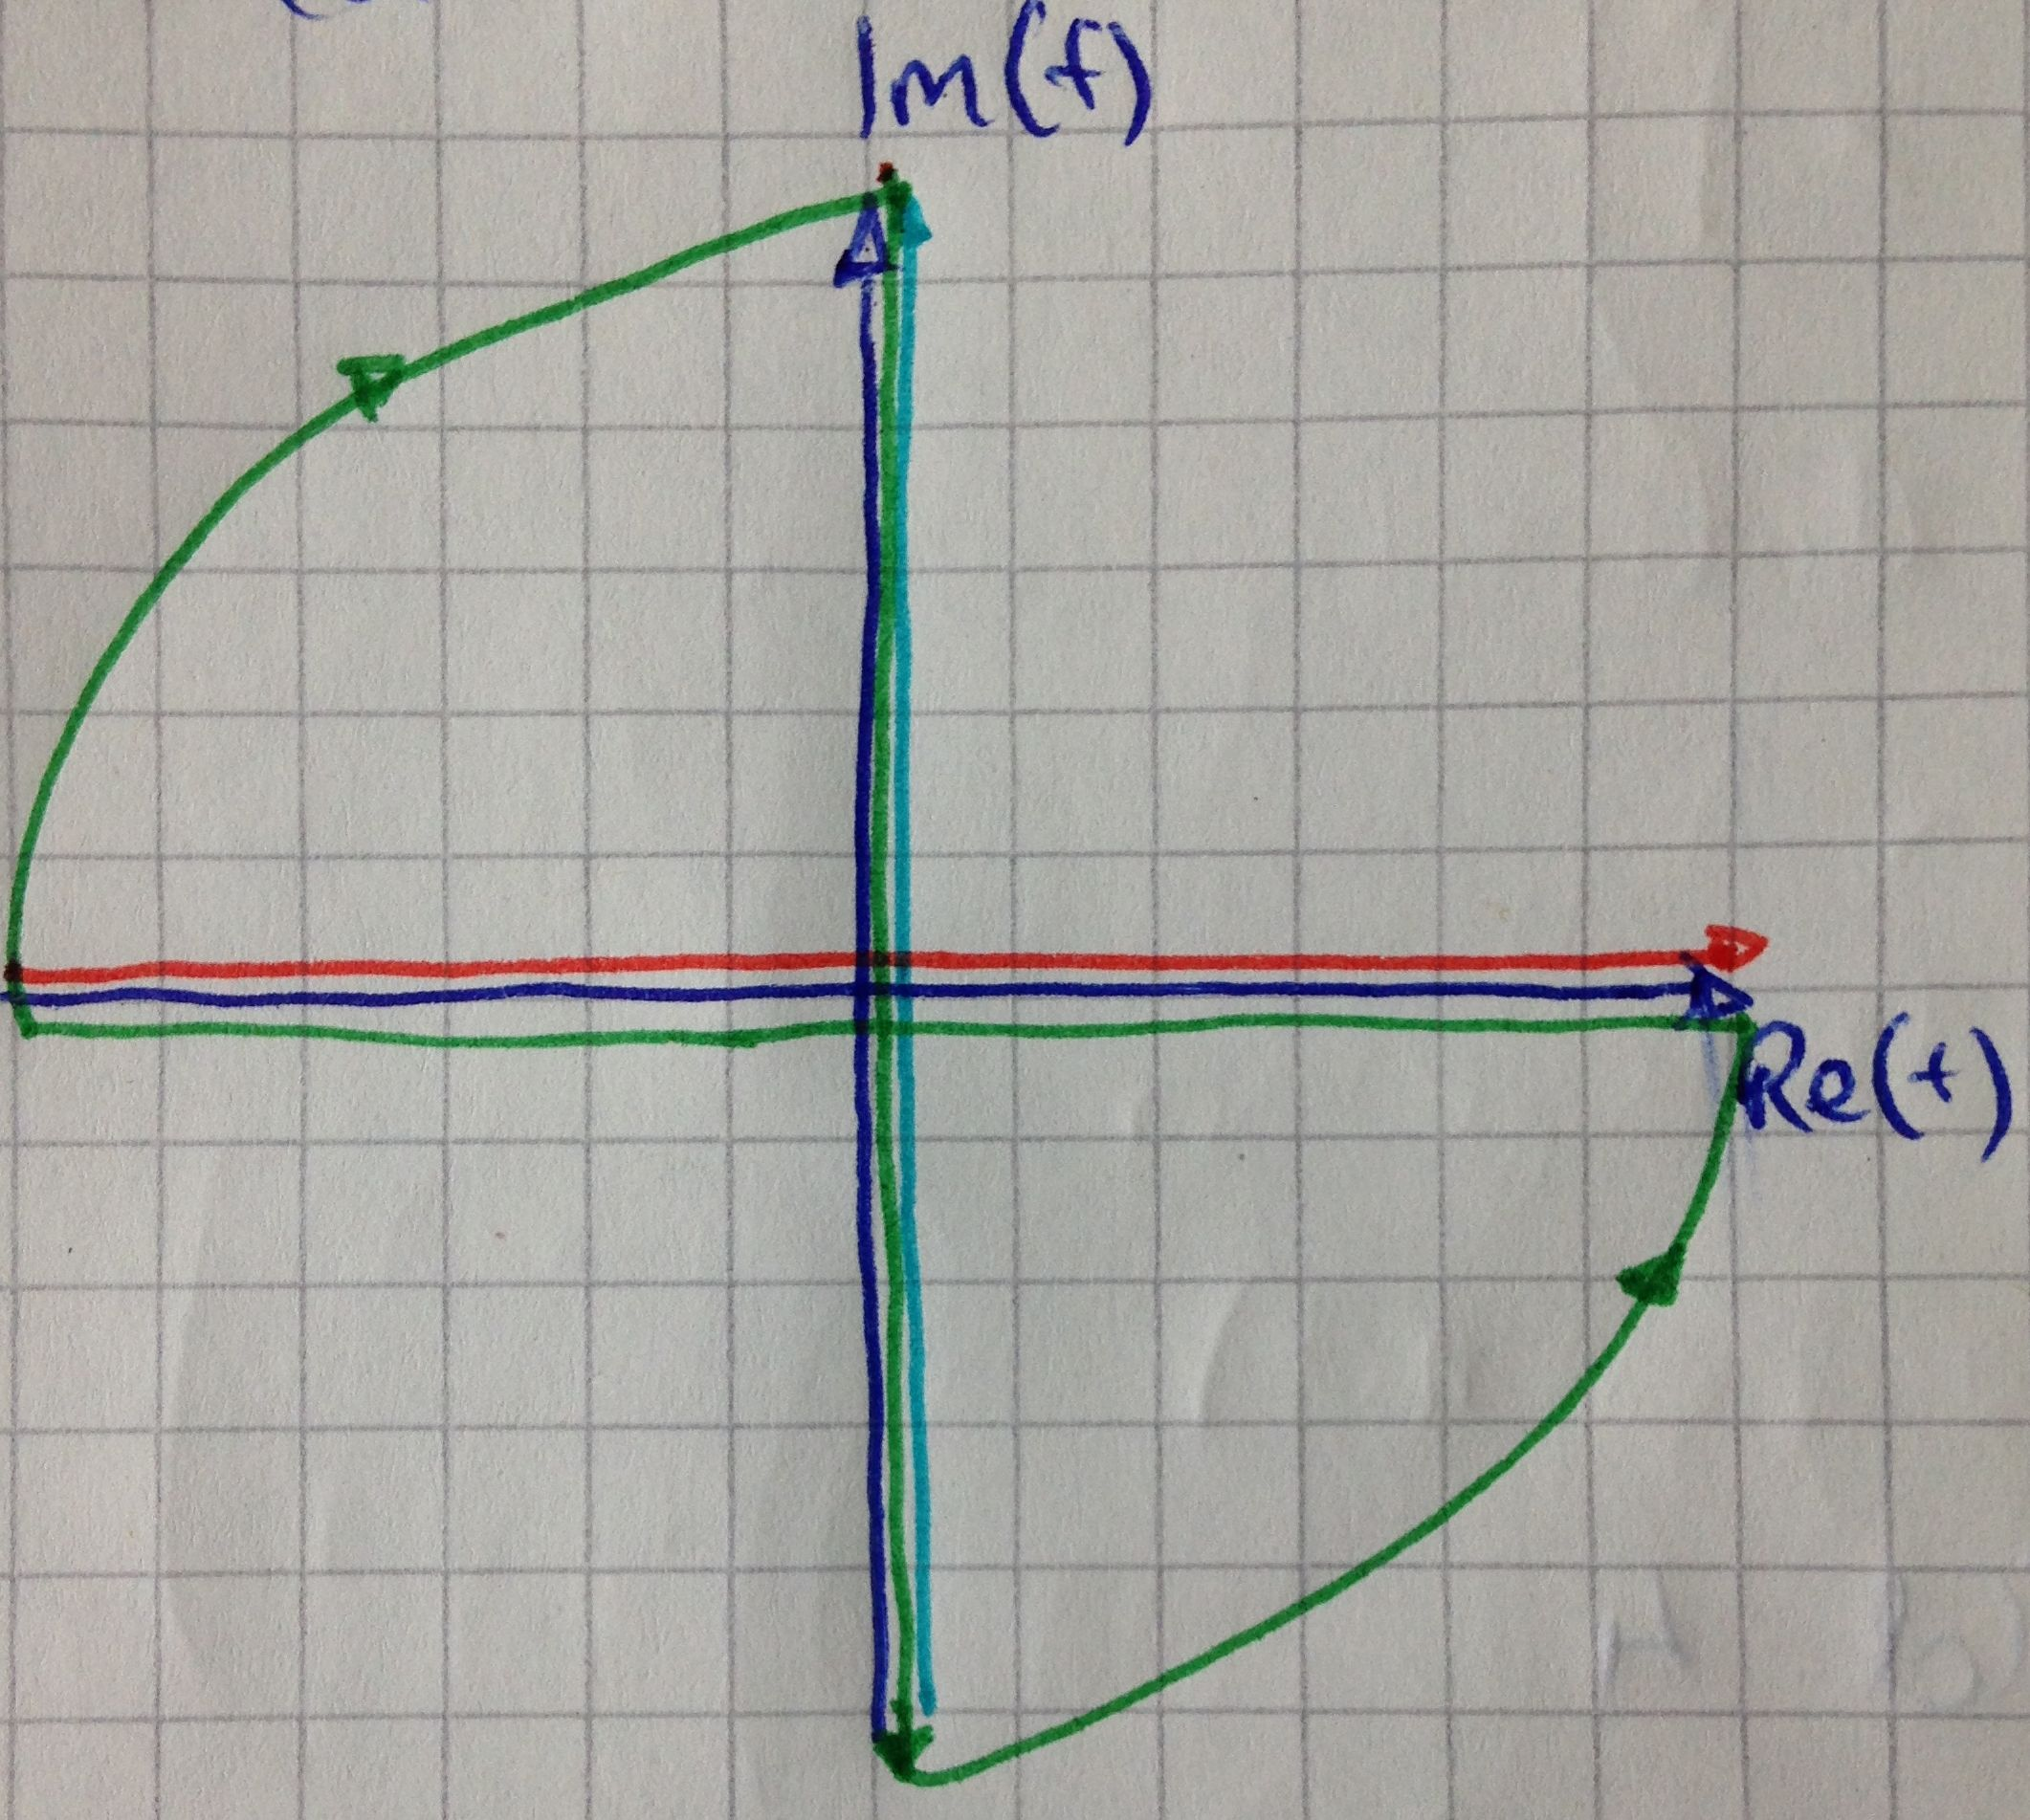
\includegraphics[width=10cm]{euklidisches_Pfradintegral1}
			\end{center}
			\end{figure*} 
\FloatBarrier
Annahmen:
	\begin{enumerate}[(1)]
		\item Kein Pol in 2. und 4. Quadranten
		\item $\int_{\text{untere grüne Kurve}} \diff t~L = \int_{\text{obere grüne Kurve}} \diff t ~L = 0$
	\end{enumerate}
	\begin{align*}
	\Rightarrow \int_{\text{über ganze grüne Kurve}} \diff t ~L = 0 = \int_{-\infty}^{\infty} \diff t ~L + \int_{i\infty}^{-i\infty} \diff t ~L
	\end{align*}	
	\begin{align*}
		S &= \int \limits_{-\infty}^{\infty} \diff t ~L = \int \limits_{-i\infty}^{i\infty} \diff t ~L = i \int \limits_{-\infty}^{\infty} \diff \tau \cdot L \\
		\tau &= + it \\
		e{\frac{i}{\hbar} S} &= e^{\frac{\int_{-\infty}^{\infty}\diff \tau ~L}{\hbar}} =
		\exp\left(-\frac{1}{\hbar} \int_{-\infty}^{\infty} \diff \tau ~L_E(\vec{r}, \frac{\partial \vec{r}}{\partial \tau})\right)
	\end{align*}
mit $\tau = i t$ Euklidische Zeit \\
$L_E = -L$: Euklidische Lagrangefunktion
	\begin{align*}
		\frac{\partial}{\partial t} &= i \frac{\partial}{\partial \tau} \\
		\frac{1}{2} m \left(\frac{\diff \vec{r}}{\diff t}\right)^2 &=
		-\frac{1}{2} m \left(\frac{\diff \vec{r}}{\diff \tau}\right)^2 \\
		L_E &= - L = \frac{1}{2} m \left(\frac{\diff \vec{r}}{\diff \tau}\right)^2 + V(\vec{r})
	\end{align*}
Euklidische Wirkung:
	\begin{align*}
		S_E &= \int_{-\infty}^{\infty} \diff \tau ~L_E
	\end{align*}
	\begin{align*}
		{}_H\braket{x_f; \tau= \infty | x_i ; \tau= -\infty}_H &= 
		\int [\diff x] e^{-\frac{S_E[x(t)]}{\hbar}}
	\end{align*}
$\tau$ ist keine ``echte'' Zeit mehr.\\

	\begin{tabular}{l l}
		Vorteil: & Keine komplexen Phasen. Nicht-klassische Pfade werden exponentiell \\
		 & mit $e^{-\frac{S_E}{\hbar}}$ unterdrückt.\\
		 Nachteil: & Wir haben Information über zeitliche Entwicklung verloren. \\
		 NB: & Pfadintegrale lassen sich auch in euklidischer Raumzeit herleiten:\\
		 & Transferoperator: 
		 $T_E = \exp\left(-\frac{a}{2\hbar} V(\hat{x})\right) \exp\left(-\frac{a}{\hbar} \frac{\hat{p}^2}{2m}\right) \exp\left(-\frac{a}{2\hbar} V(\hat{x})\right)$\\
		 Vorteil 2: & $\int [\diff x] e^{-\frac{S[x(t)]}{\hbar}}$ lässt sich als relative Wahrscheinlichkeit (Maß) interpretieren
	\end{tabular}